\documentclass[runningheads,a4paper]{llncs2e/llncs}

\setcounter{tocdepth}{3}
\usepackage{graphicx}

\usepackage{amsmath}
\usepackage{amsfonts}
\usepackage{amssymb}

\usepackage[utf8]{inputenc}

%\usepackage{amsmath,amsthm,amssymb}
\usepackage{color}
\usepackage{nicefrac}
%\usepackage{stmaryrd} % for \llbracket and \rrbracket
%\usepackage{graphicx}
\usepackage{multirow}
\usepackage{rotate}
\usepackage{wrapfig}
%\usepackage{hyperref}
%\usepackage{mathtools}
%\usepackage[titletoc]{appendix}
\usepackage{subcaption}

%%%%%%
% Comment
%
\newif\ifcommentson\commentsonfalse
%\newif\ifcommentson\commentsontrue
\def\mywidth{.9}        %\def\mywidth{.45}
\def\mywidthRep{.8} %\def\mywidthRep{.43}
\ifcommentson
\newcommand{\commentAA}[1]{\begin{center} \parbox{\mywidth\textwidth}{\textbf{\textcolor{black}{Comment A.}} \textcolor{red}{#1 }}\end{center}}
\newcommand{\commentAB}[1]{\begin{center} \parbox{\mywidth\textwidth}{\textbf{\textcolor{black}{Comment B.}} \textcolor{red}{#1} }\end{center}}
\newcommand{\commentMA}[1]{\begin{center} \parbox{\mywidth\textwidth}{\textbf{\textcolor{black}{Comment M.}} \textcolor{red}{#1} }\end{center}}
%
\newcommand{\replyAA}[1]{\begin{center} \parbox{\mywidthRep\textwidth}{\textbf{Reply A.} \textcolor{blue}{#1} }\end{center}}
\newcommand{\replyAB}[1]{\begin{center} \parbox{\mywidthRep\textwidth}{\textbf{Reply B.} \textcolor{blue}{#1} }\end{center}}
\newcommand{\replyMA}[1]{\begin{center} \parbox{\mywidthRep\textwidth}{\textbf{Reply M.} \textcolor{blue}{#1} }\end{center}}
%
\newcommand{\commentA}[1]{\marginpar{\footnotesize \color{red} {\bf A:} \textsf{\scriptsize #1}}}
\newcommand{\commentB}[1]{\marginpar{\footnotesize \color{red} {\bf B:} \textsf{\scriptsize #1}}}
\newcommand{\commentM}[1]{\marginpar{\footnotesize \color{red} {\bf M:} \textsf{\scriptsize #1}}}
%
\newcommand{\replyA}[1]{\marginpar{\footnotesize \color{blue} {\bf A:} \textsf{\scriptsize #1}}}
\newcommand{\replyB}[1]{\marginpar{\footnotesize \color{red} {\bf B:} \textsf{\scriptsize #1}}}
\newcommand{\replyM}[1]{\marginpar{\footnotesize \color{red} {\bf M:} \textsf{\scriptsize #1}}}
%
\else
\newcommand{\commentAA}[1]{}
\newcommand{\commentAB}[1]{}
\newcommand{\commentMA}[1]{}
\newcommand{\replyAA}[1]{}
\newcommand{\replyAB}[1]{}
\newcommand{\replyMA}[1]{}
\newcommand{\commentA}[1]{}
\newcommand{\commentB}[1]{}
\newcommand{\commentM}[1]{}
\newcommand{\replyA}[1]{}
\newcommand{\replyB}[1]{}
\newcommand{\replyM}[1]{}
\fi
%%%%%%

% Macros for this paper specifically.
%Macros for changing after review
%\newcommand{\review}[1]{\textcolor{blue}{#1}} 
\newcommand{\review}[1]{#1}
\newcommand{\cutout}[1]{\textcolor{red}{#1}}
%\newcommand{\cutout}[1]{}


%\newcommand\Cite[1]{[\textbf{\color{red}{#1}}]} % Use for a citation to be filled-in later.
\newtheorem{Theorem}{Theorem}
\newtheorem{Lemma}[Theorem]{Lemma}
\newtheorem{Corollary}[Theorem]{Corollary}
\newtheorem{Proposition}[Theorem]{Proposition}
\newtheorem{Conjecture}[Theorem]{Conjecture}
\newtheorem{Definition}[Theorem]{Definition}
\newtheorem{Example}[Theorem]{Example}

\newcommand{\calw}{\mathcal{W}}
\newcommand{\calx}{\mathcal{X}}
\newcommand{\caly}{\mathcal{Y}}
\newcommand{\calz}{\mathcal{Z}}
\newcommand{\calf}{\mathcal{F}}
\newcommand{\calg}{\mathcal{G}}

\newcommand{\cupdot}{\mathbin{\mathaccent\cdot\sqcup}}
%\newcommand{\hoper}{{}_p\oplus}
\newcommand{\hchoice}[1]{\;{{}_{\mathit{#1}}{\oplus}}\;} % operator to be used among parameters: it gives nice spacing.
\newcommand{\hchoiceop}[1]{{}_{\mathit{#1}}{\oplus}} % name of the operator, to be used when no paramaters are needed.
%\newcommand{\voper}{{}_{p}\cupdot}
\newcommand{\vchoice}[1]{\;{{}_{\mathit{#1}}{\cupdot}}\;} % operator to be used among parameters: it gives nice spacing.
\newcommand{\vchoiceop}[1]{{}_{\mathit{#1}}{\cupdot}} % name of the operator, to be used when no paramaters are needed.
\newcommand{\reals}{\mathbb{R}}
\newcommand{\dist}{\mathbb{D}}
\newcommand{\imp}{\Rightarrow}
\newcommand{\conc}{\otimes}

\newcommand{\qm}[1]{``#1''}

\newcommand{\hyperc}[2]{[#1 , #2]} % Hyper [\pi > C] created by pushing a prior \pi through a channel C
\newcommand{\ggid}{g_{\mathit{id}}} % g_id gain function
\newcommand{\vgid}{V_{\gid}} % V_{g_{id}}, the g-vulnerability corresponding to g_id
\newcommand{\pchoice}[1]{\;{{}_{\mathit{#1}}\oplus}\;}%redefined by Catuscia probabilistic choice
\newcommand{\zeromat}{\hat{0}}
\newcommand{\nullchannel}{\overline{0}} % Null channel.
\renewcommand{\equiv}{\approx}

\usepackage[bookmarks=false,linktocpage=true,colorlinks=false]{hyperref} % For use of \href{}.

% vulnerabilities
\newcommand{\vg}{V_{g}} % name of g-vulnerability
\newcommand{\priorvg}[1]{\vg\left[#1\right]} % prior g-vulnerability
\newcommand{\postvg}[2]{\vg\left[#1,#2\right]} % posterior g-vulnerability
\newcommand{\vf}{\mathbb{V}} % name of generic vulnerability function
\newcommand{\priorvf}[1]{\vf\!\left[#1\right]} % prior generiic vulnerabiltiy fuction
\newcommand{\postvf}[2]{\vf\!\left[#1,#2\right]} % posterior generiic vulnerabiltiy fuction

% math
\newcommand{\eqdef}{\ensuremath{\stackrel{\mathrm{def}}{=}}}


\begin{document}

\mainmatter  % start of an individual contribution

% first the title is needed
\title{Proposta de Projeto Orientado em Computação}
% a short form should be given in case it is too long for the running head
%\titlerunning{POC I}

% the name(s) of the author(s) follow(s) next
%
% NB: Chinese authors should write their first names(s) in front of
% their surnames. This ensures that the names appear correctly in
% the running heads and the author index.
\author{Artur Duarte Penna Vaz\\
Orientador: Mário S Alvim}
%
\authorrunning{Artur Vaz}
% (feature abused for this document to repeat the title also on left hand pages)

% the affiliations are given next; don't give your e-mail address
% unless you accept that it will be published
\institute{Universidade Federal de Minas Gerais, Brazil}

%
% NB: a more complex sample for affiliations and the mapping to the
% corresponding authors can be found in the file "llncs.dem"
% (search for the string "\mainmatter" where a contribution starts).
% "llncs.dem" accompanies the document class "llncs.cls".
%

\toctitle{Lecture Notes in Computer Science}
\tocauthor{Authors' Instructions}
\maketitle
\newpage
\section{Introdução}
\label{sec:introducao}
% Modelo americo/mario de intro
Proteger informação sensível do público é um objetivo importante de segurança. O campo do Fluxo Quantitativo de Informação(QIF) se preocupa com em quantificar o quanto de informação sensível um sistema vaza, e tem sido muito ativo na ultima decada [1]-[X]. 

A representação do sistema é chamada de \emph{Canal} e é a distribuição de probabilidade das saidas de cada entrada, essa definição modela o comportamento do sistema.
O problema com a modelagem é que intuitivamente a abordagem é pensar no sistema como uma coisa só, que é suficiente para sistemas simples e pequenos mas para sistemas robustos não é uma tarefa trivial.

A partir disso, foi proposto uma abordagem aproximativa que modela o canal a partir da composição de partes do sistema e é proposto operadores que capturam as interações que ocorrem entre os componentes. %Falar sobre a abordagem tradicional
Essa abordagem simplifica o processo de modelagem. % Faz mais alguma coisa?

O objetivo desse projeto é comparar a análise de fluxo de informação pela aproximação usando os operadores e pelo calculo exato no canal e modelar protocolos como composição de canais e analisar o fluxo de informação. 
Na primeira parte do Projeto Orientado em Computação será feita uma comparação do vazamento de informação em protocolos já estudados, usando as diferentes abordagens, e será implementada uma biblioteca em C++ para auxiliar esse projeto, e futuros. 
Na segunda parte novos protocolos serão analisados usando o método aproximativo.

\section{Referencial Teórico}
\label{sec:referencial_teorico}
%Apresente os conceitos pertinentes para que o leitor entenda o problema e sua importância. Nesse momento, o aluno pode não ter domínio completo dos trabalhos relacionados. Fazer um breve resumo das soluções já existentes na literatura/mercado e como elas se comparam ao trabalho proposto. No caso de trabalhos de cunho tecnológico, listar ferramentas que resolvem o mesmo problema sendo tratado.

% No framework, modelos de seguranca sao modelados como canais de informacao teorico.
% Definir canal
% 

No campo de QIF, modelos de segurança são modelados como canais de informação. Um canal é definido como uma função $C: \calx \times \caly \rightarrow \reals$ onde $\calx$ é o grupo das entradas, ou valores secretos, e $\caly$ é grupo dos outputs, ou observáveis:

$$ C(x,y) = p(y|x) $$

$C(x,y)$ é a probilidade do sistema produzir o observável $y$ dado o segredo $x$, $\forall x \in \calx$ e $\forall y \in \caly$.

Por exemplo, podemos modelar um sistema de login onde $\calx$ é o grupo de todas as possíveis senhas e $\caly$ um grupo de 2 elementos, se a senha é certa ou errada. Nesse sistema apenas um elemento é correto e o restante incorreto.
\begin{table}[h!]
\centering
\begin{tabular}{|c|c c|}
    \hline
    $C$   & Correto & Incorreto  \\
    \hline 
    $"123455"$&0&1\\
    $"123456"$&1&0\\
    \hline
\end{tabular}
\caption{Representação matricial de um canal}
\label{Tabela:1}
\end{table}
Esse exemplo é determinista e interessante para perceber a interpretação do canal porem em sistemas de segurança é comum ter varios observáveis possíveis para cada segredo.

Para entender como a informação vaza é preciso modelar também o \emph{atacante}, é assumido que o observável e o sistema é conhecido. Alem disso, o adversário pode saber um pouco sobre o segredo antes do sistema executar e é defindo como distribuição apriori $\pi$ em $\calx$, uma distribuição de probabilidades sobre os segredos. 
%Talvez remover ", uma distribuicao de probabilidades sobre os segredos."



%In the QIF framework, security models are modeled as information-theoretical channels. A channel $C: \calx \times \caly \rightarrow \reals$ where $\calx$ is the set of inputs, or secret values, and $\caly$ is the set of outputs, or observables

\section{Metodologia}
\label{sec:metodologia}
%Quais os principais passos previstos (com uma breve descrição)
%para execução do projeto? Como pretende-se abordar o problema?
%
%two parts parser
%  lexer -> parser
%
%  criando tokens eh possivel categorizar de antemao todos os elementos da eq e em seguida alimentar o parser de forma mais simples
%
%good source: https://tomassetti.me/parsing-in-python/
%
%############################################################
%ROADMAP:
%  simple lexer = done?
%  parser          = done
%  old metrics
%  new metrics
%  composition operators
%  make a better lexer :)

O projeto consiste em implementar as ferramentas e analisar a diferença entre a aproximação do vazamento, usando os operadores, e o cálculo exato feito diretamente no canal.

A primeira parte do projeto é implementar uma biblioteca em C++ que contenha o ferramental para análise. Essa biblioteca vai conter:

\begin{itemize}
  \item{Estrutura do canal}
  \item{Utilidades para a classe do canal}
  \item{Métricas antigas}
  \item{Métricas novas}
  \item{Operadores de composição}
%\item{Parser}
\end{itemize}

O canal vai ser definido como uma classe onde as métricas e os operadores são métodos. 
Será implementado algumas utilidades, por exemplo, gerar um canal aleatorio, verificar se canais são compatíveis, etc.
%Um Parser foi implementado para permitir operações de composição com vários canais de forma simples. 

A segunda parte é analisar a efetividade dos operadores de composição.
Existem dois protocolos de segurança, \emph{Dining Cryptographers} e \emph{Crowds}, comuns na literatura de QIF que podem ser usados para comparar o vazamento de informação usando os métodos diferentes.
%Obter um canal não é trivial e os operadores de composição permitem uma nova abordagem a esse problema, com eles é possível modelar partes do sistema e compor o canal. 
%Essa abordagem é natural para sistemas de segurança pois muitas vezes são compostos de entidades separadas que se relacionam.


\section{Resultados Esperados}
\label{sec:resultados}
%O que se pretende obter ao final do trabalho?
Ao final do POC I teremos uma implementação para o framework de QIF, com metricas e operações, que por sí só já em um boa contribuição para futuras pesquisas. 
Além disso, mostrar que metodos aproximativos são uma alternativa viável para modelar sistemas de segurança contribui para a modelagem de sistemas cada vez maiores e complexos.

No POC II é esperado expandir a quantidade de sistemas de segurança modelados e analisados na literatura.

\section{Etapas e Cronograma}
\label{sec:etapas}
%Descrever o cronograma previsto para a realização dos passos definidos na Metodologia com resolução em nível de semanas.
%Roadmap
%
%- Implementação
%  - Parser 		OK
%  - Estrutura 		OK
%  - Utilidades 		WIP
%	09/04 -> 15/04
%  - Metodos Antigos	0%
%	16/04 -> 23/04
%  - Metodos Novos	0%
%	23/04 -> 29/04
%  - Operadores		0%
%	30/04 -> 06/04
%- Comparacao dos metodos
%  - Modelagem e analise usando metodo tradicional
%	07/05 -> 13/05
%  - Modelagem e analise usando metodo aproximativo
%	14/05 -> 20/05
%- Restantes
%  - Escrever o relatorio
%  - Poster
%  - Apresentacao parcial e final
%  - Bugfixes e melhorias

O cronograma(Fig. 1) foi definido dividindo as etapas em blocos de semana, e pelo planejado a implementação e a análise deve estar pronta na época da apresentação parcial. O parser já foi implementado.

\begin{figure}[h]
\centering
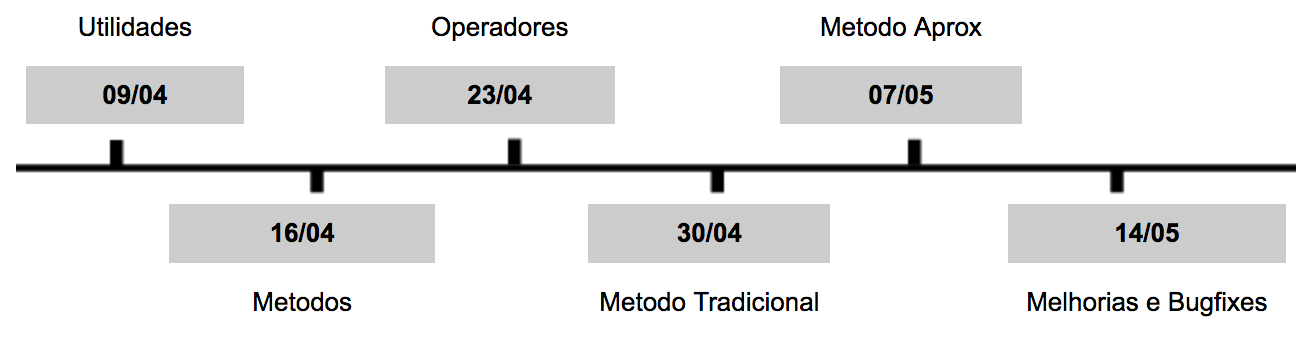
\includegraphics[width=\textwidth]{roadmap.png}
\caption{Cronograma}
\end{figure}

Do dia 14/05 para frente será reservado para melhorar a usabilidade da biblioteca e resolver eventuais problemas.


\bibliographystyle{abbrv}
\bibliography{references,short}

%\appendix
%\input{password-example}
%\input{working-notes}
\end{document}
